\subsection{Data Collection}
\label{subsec:datacollection}

For over two weeks, we deployed a data collection system to observe empirical temporal information about lifetime and bandwidth consumption in Tor circuits.
Our objective was to have a deeper understanding of typical Tor usage and whether such usage could benefit from our channel-based payment system.
For example, these measurements might capture the distribution of type and magnitude of potential premium traffic.
We classify the traffic type based on the service connection port.
In addition to the standard ports 80 and 443 used for web traffic, we aggregated data from some other families, including the WHOIS protocol~\cite{daigle2004whois} and RWHOIS~\cite{williamson1994referral} from ports 43 and 4321, respectively.
By specifying a reduced exit policy, we can identify traffic patterns according to known types.

\begin{figure*}[t] \centering
  \begin{subfigure}[t]{0.47\textwidth} \centering\centering
    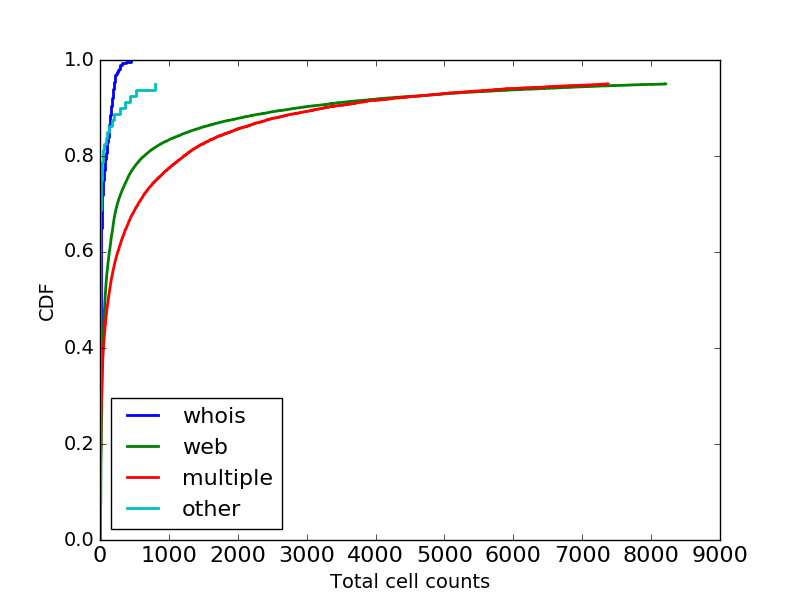
\includegraphics[width=0.7\textwidth]{images/totcellcountscdf.png}
    \caption{Total Counts --- Distribution of circuit size with respect to the total number of cells processed}
    \label{fig:statsb}
  \end{subfigure}
  \begin{subfigure}[t]{0.47\textwidth} \centering
    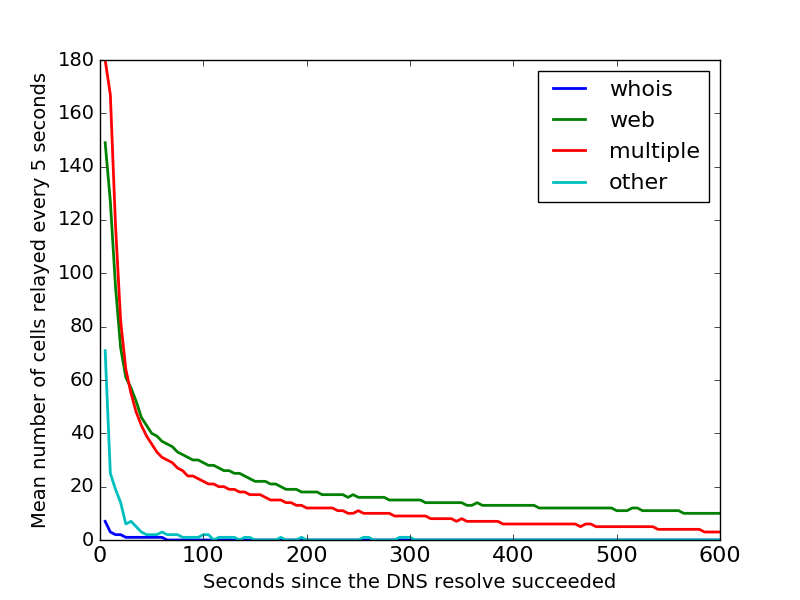
\includegraphics[width=0.7\textwidth]{images/exitmeasurement.png}
    \caption{Time Profile --- Average distribution of traffic across circuit lifetime beginning with the first DNS request.}
    \label{fig:statsa}
  \end{subfigure}
  \caption{Data collection from 5 old and stable exit relays with a cumulative bandwidth of $\approx$50 MiB/s}
  \label{fig:stats}
\end{figure*}

\paragraph*{Efforts to preserve users privacy}

To ensure ethical experimentation, we contacted the Tor research safety board~\cite{torsafety} and used their feedback to inform our data collection process.~\footnote{E.g.
avoid writing metadata from any specific flow or circuit to disk.}
We collected data from five old and stable exit relays with a total bandwidth of 50 MiB/s, stripped the origin metadata, aggregated it in memory, and stored it on a central server into bins of configurable size for each traffic type.
The data only covers circuits that are ``active'' from the perspective of the exit relay, in other words, circuits that have received a connection request to an IP address on the internet.
Once we collected enough data (1600 circuits) from a single type, we saved the information on the disk, cleared the relay memory, and resumed a new session.
Crucially, we did not record information linked to any single particular user flow on disk.
The final result contained only aggregated data with following two pieces of information for each pool:

\begin{itemize}
\item \textbf{Time Profile}: The total number of inbound and outbound cells in each 5-second time interval. Tracking begins after the conclusion of a successful DNS request.
\item \textbf{Total Counts}: The total amount of cells processed by a circuit.
  We aggregate this information by taking the mean of fixed-size nearest neighbor bins.
\end{itemize}

\paragraph*{Observations}

Our measurements successfully captured several essential pieces of information for the design and justification of moneTor.
For example, one crucial task is to determine the number of potential users that could benefit from paid traffic.
From Figure~\ref{fig:statsb}, we observe that $\approx 82\%$ of circuits carrying only web traffic exchanged less than 1000 cells.
While we cannot deduce any statements about users, we can speak to the fraction of circuits that may benefit from a payment channel in the Tor network, since around $50\%$ of them do not carry data and less than $17\%$ of them carry at least one web page.
The remaining $18\%$ would appear to be better candidates for moneTor.

It is also evident from Figure~\ref{fig:statsa} that most of the traffic is usually carried within the first few tens of seconds regardless of traffic type.
From that result, we believe that the reliability of payment is critical within the first few seconds, especially from a relay perspective.
This result highlights our choice to extend Bolt to offer high fairness.
Furthermore, the front-loaded distribution curve indicates a need to establish available payment channels as soon as the user opens a circuit.
As a result, we base our design upon a preemptive circuit build strategy, which effectively eliminates channel setup/establish latency in the average case.
